 
\section{Preliminary Results}
\label{sec:results}

%
% RESULTS TODO
%
% need to motivate optimization workflow and plans
% current ideas not bad, need more
%
%

The computer simulations in this proposal study are intended to discover
the optimal solar vortex system configuration for a range of scenarios
and system sizes. 
This section contains discussions of the preliminary simulation results 
to motivate that the existing simulation capability is sufficiently well
developed and understood to permit an efficient exploration of the SoV
configuration space. 
This section begins with a discussion of the structure of solutions from
a representative case with no ambient winds, the ``thermal only''
situation. Next, a case with strong ambient horizontal winds (``Wind'')
is discussed. Finally, the results from a series of runs are shown to
demonstrate heuristic by which incremental optimization of the system
configuration will be conducted. 

%The results of these optimized configurations will be used as input
%for the design of a prototype to be tested in Mesa, Arizona this
%summer. 

% \todo{add photo}
  % \begin{figure}[!htb]
  %  \begin{center}
  %   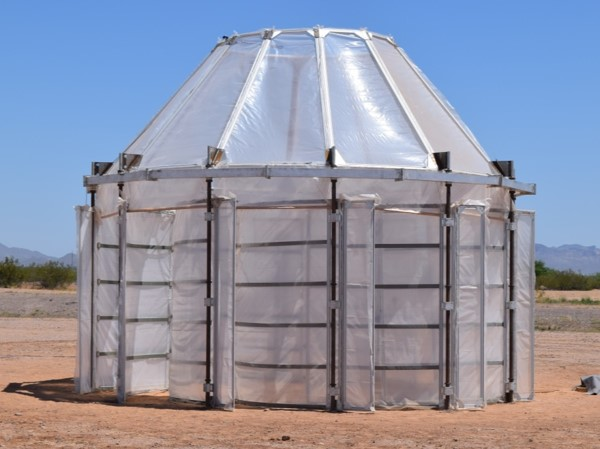
\includegraphics[width = 12 cm]{figs/sov_field}
  %   \caption{A photo of the field configuration, during the June 2015
  %   Field Test.}
  %   \label{fig:field_real}
  %  \end{center}
  % \end{figure}

\subsection{Thermal Only}

While ambient winds in the field impact system performance, it is
also illuminating to consider an idealized scenario with natural convection
driven only by thermal instabilities. Simulations of this baseline,
thermal-only flow are intended to ensure the SoV apparatus to form a
strong thermal plume even in the absence of wind. 
%After a system is
%engineered to form a strong thermal plume, we can investigate to ensure
%that the existing thermal vortex will be strengthened by the addition of
%winds. %\todo{do I need image of vanes? and explain how calculated}

\begin{figure}[htb]
\centering
\begin{minipage}{0.45\textwidth}
\centering
 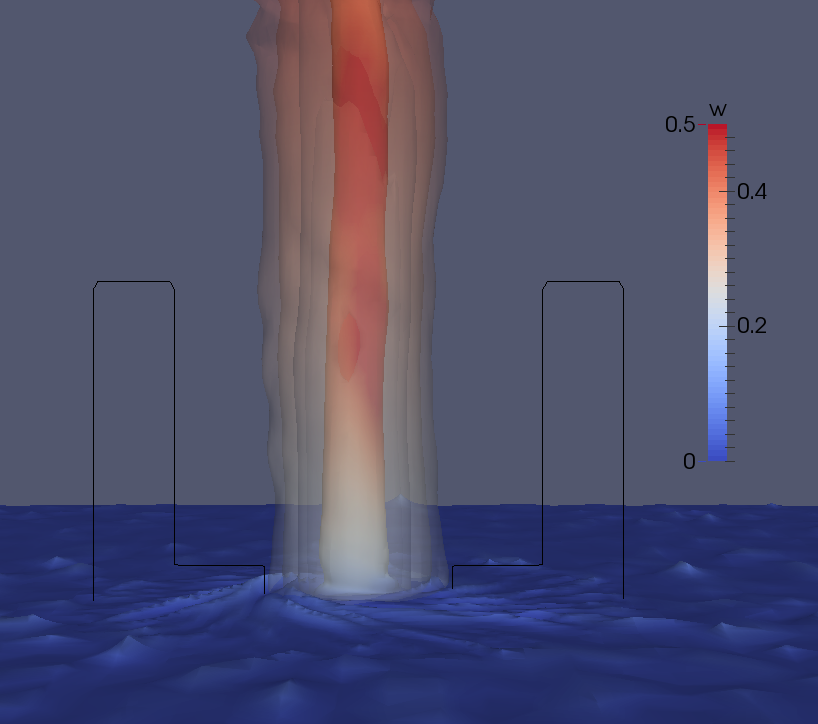
\includegraphics[width=.8\linewidth]{figs/3d}
 \caption{Isocountours of the inner thermal core
  visible through semi-transparent contour around azimuthal velocity,
  colored by vertical velocity. An outline of the region of virtual
  vanes has been drawn.}
 \label{fig:thermal}  
\end{minipage}\hfill
\begin{minipage}{0.45\textwidth}
\centering
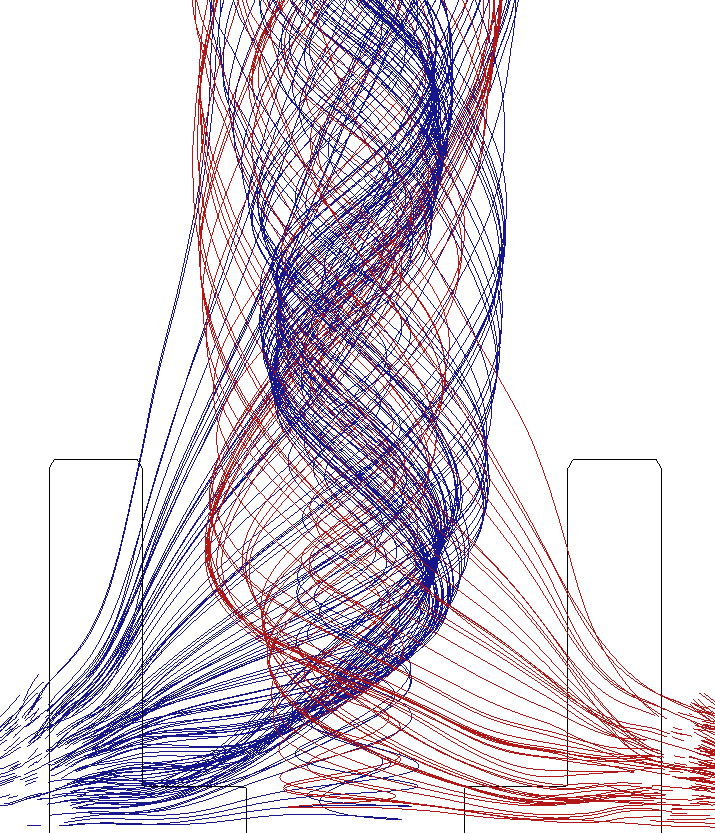
\includegraphics[width =0.8\textwidth]{figs/entrainment}
\caption{Fluid entrainment around the apparatus. An outline of the
  virtual vanes are drawn to show the region of forcing.}
 \label{fig:entrain}  
\end{minipage}
\end{figure}



% \begin{figure}[htb]

%  \begin{subfigure}{.55\textwidth}
%   \centering
%   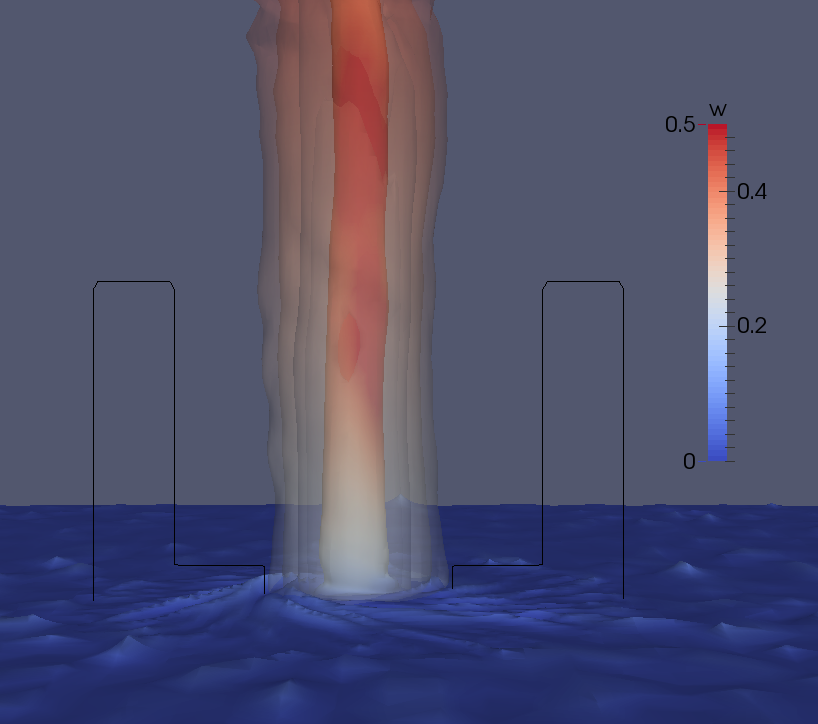
\includegraphics[width =0.7\textwidth]{figs/3d}
%   \caption{Isocountours of the inner thermal core
%   visible through semi-transparent contour around azimuthal velocity,
%   colored by vertical velocity. An outline of the region of virtual
%   vanes has been drawn.}
%   \label{fig:thermal}  
%  \end{subfigure}%
%  \begin{subfigure}{.4\textwidth}
%   \centering
%   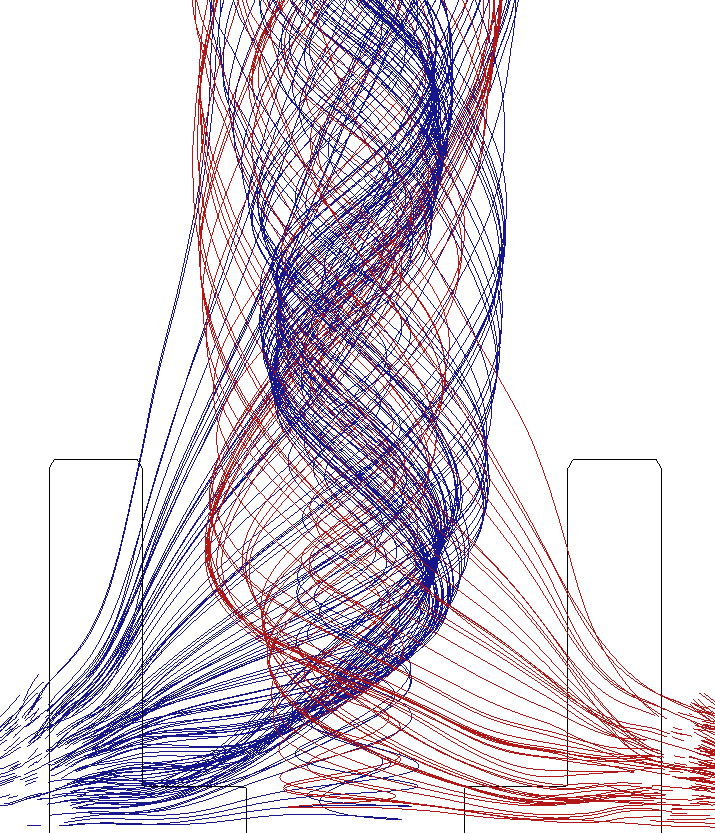
\includegraphics[width =0.8\textwidth]{figs/entrainment}%
%   \caption{Fluid entrainment around the apparatus. An outline of the
%   virtual vanes are drawn to show the region of forcing.} 
%   \label{fig:entrain}  
%  \end{subfigure}%
% \end{figure}

In this subsection a representative case of an optimized thermal-only SoV
configuration is presented.\todo{what are the conditions of this case} 
The results shown are the averages of fifty snapshots of the solution 
taken over the course of ten minutes. In general,
the averaging times are selected to be approximately 20 to 30 wash-out 
times, where a
wash-out is defined as the time required for a particle at the base of
the apparatus to flow out through the top boundary. The energy flux
through the top of the vanes for this case is about 53 watts. The solution
demonstrates several features characteristic of naturally occurring dust
devils. Figure \ref{fig:thermal} shows that there is a tight,
coherent thermal plume roughly the same size as the inner diameter of the
lower vanes. As anticipated, this hot flow is acting like a chimney,
generating a large vertical velocity which in turn entrains air from the outside.
An image of the entrainment is shown in figure\ref{fig:entrain}\todo{fix
text of this image}. The image was created by tracking particles as they
convect through the device. One can observe a tight inner vortex with
significant azimuthal velocity as well as a broader region of entraining
fluid through the upper tier of vanes. 

\begin{figure}[htb]

 \begin{subfigure}{.5\textwidth}
  \centering
  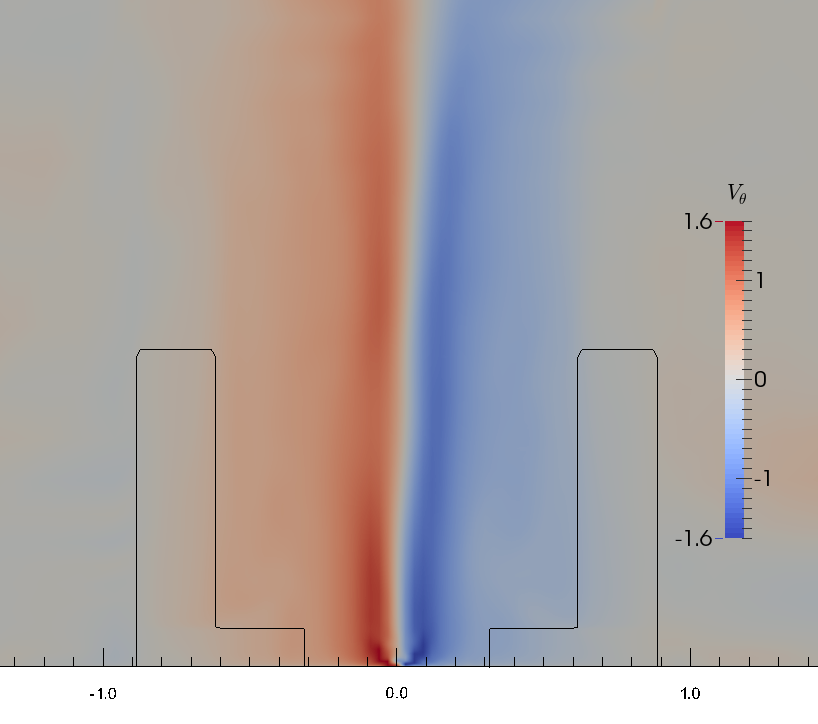
\includegraphics[width=.75\linewidth]{figs/vt}
  \caption{Azimuthal Velocity}
  \label{fig:vt-to}
 \end{subfigure}%
 \begin{subfigure}{.5\textwidth}
  \centering
  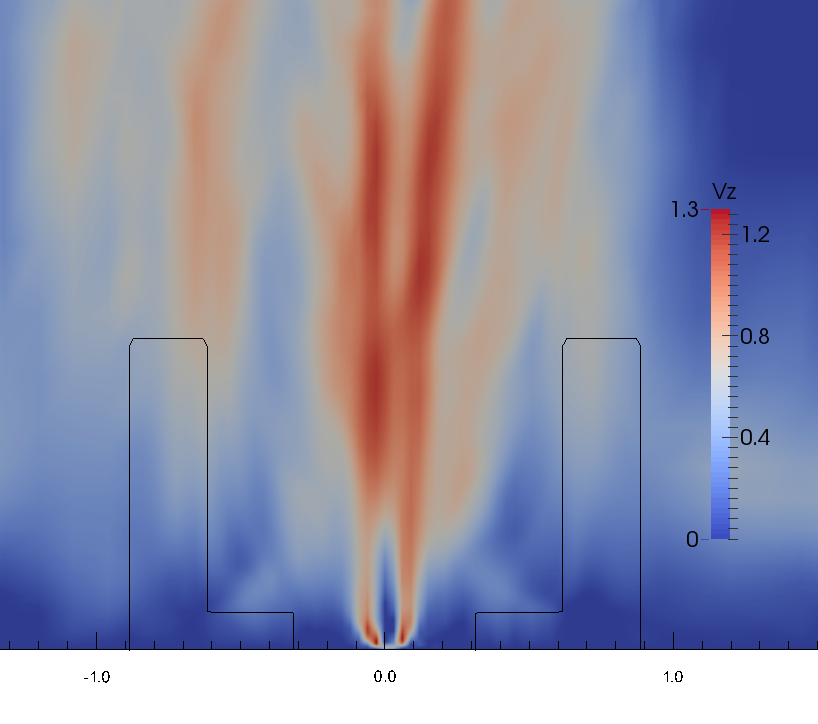
\includegraphics[width=.8\linewidth]{figs/vz}
  \caption{Vertical Velocity}
  \label{fig:vz-to}
 \end{subfigure}%


 \begin{subfigure}{.5\textwidth}
  \centering
  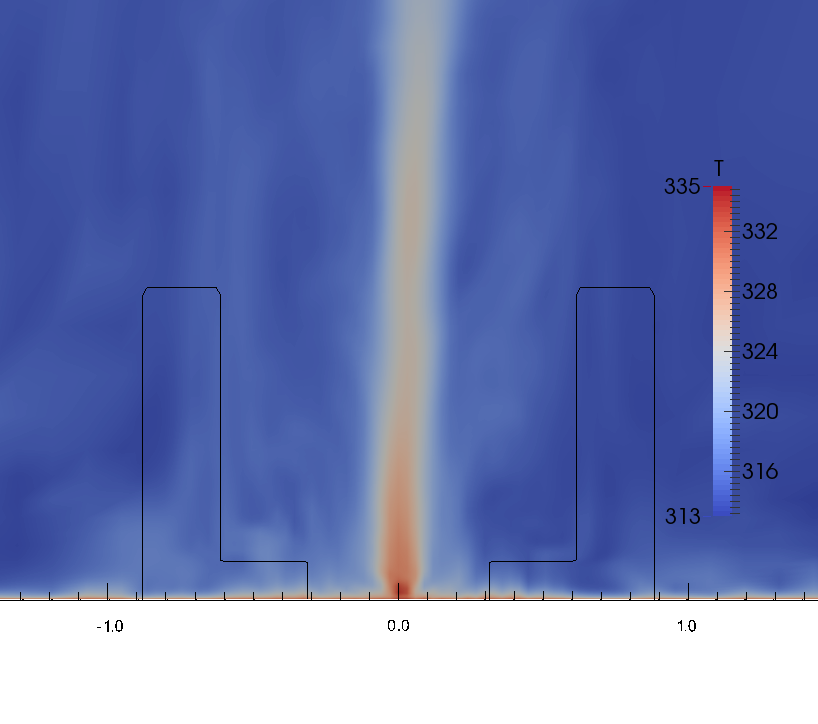
\includegraphics[width=.85\linewidth]{figs/t}
  \caption{Temperature}
  \label{fig:t-to}
 \end{subfigure}%
 \begin{subfigure}{.5\textwidth}
  \centering
  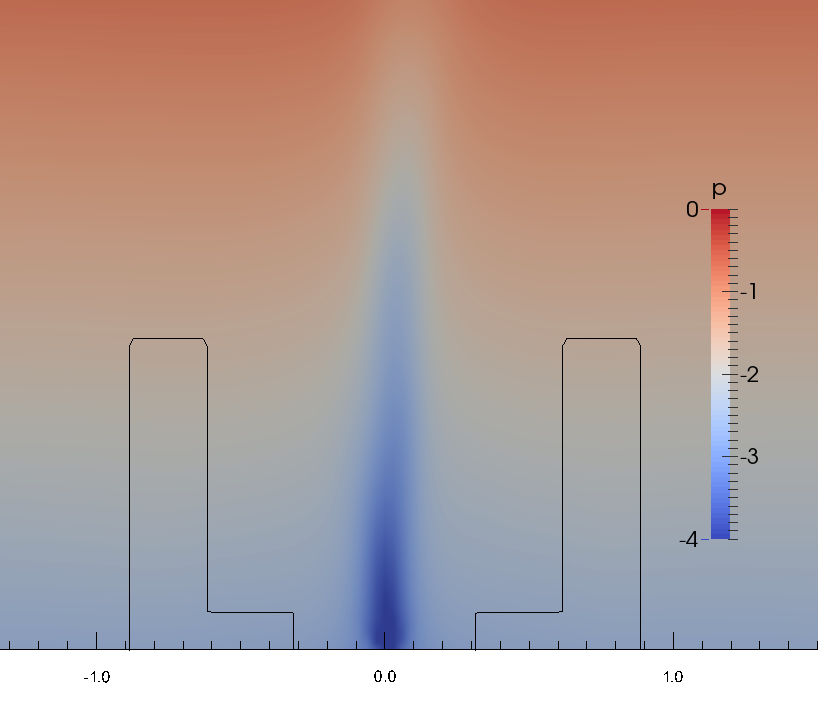
\includegraphics[width=.75\linewidth]{figs/p}
  \caption{Pressure}
  \label{fig:p-to}
 \end{subfigure}%

 \caption{Vertical slices through the center of the device for the thermal-only cases. Black lines 
   indicate the location of the vanes.}
 \label{fig:to-vert}
\end{figure}

%
%
%
Figure \ref{fig:to-vert} depicts several vertical slices through the SoV
for various state variables. One can see that there is a tight core
vortex with azimuthal and vertical velocities of several meters per
second. The tight vortex region coincides with a high temperature, low
pressure core region. The rapidly rotating air near the center induces
a low pressure core, as observed in real dust devils.
On the vertical velocity plot, notice that a small
downward flow region has formed in the middle of the vortex. 

\begin{figure}[htb]

 \begin{subfigure}{.5\textwidth}
  \centering
  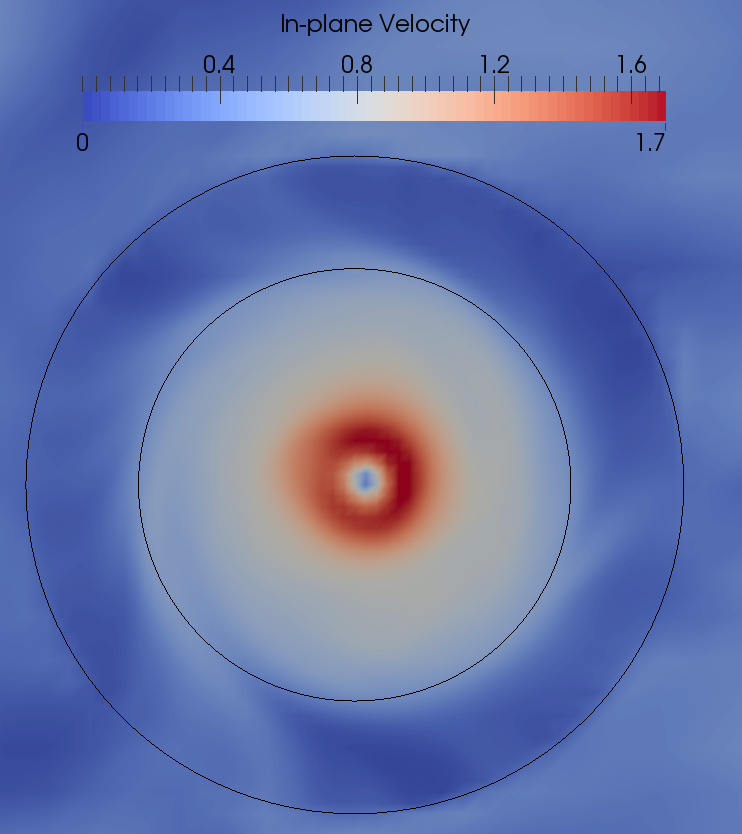
\includegraphics[width=.75\linewidth]{figs/vt_hor}
  \caption{Azimuthal Velocity}
  \label{fig:vt-to}
 \end{subfigure}%
 \begin{subfigure}{.5\textwidth}
  \centering
  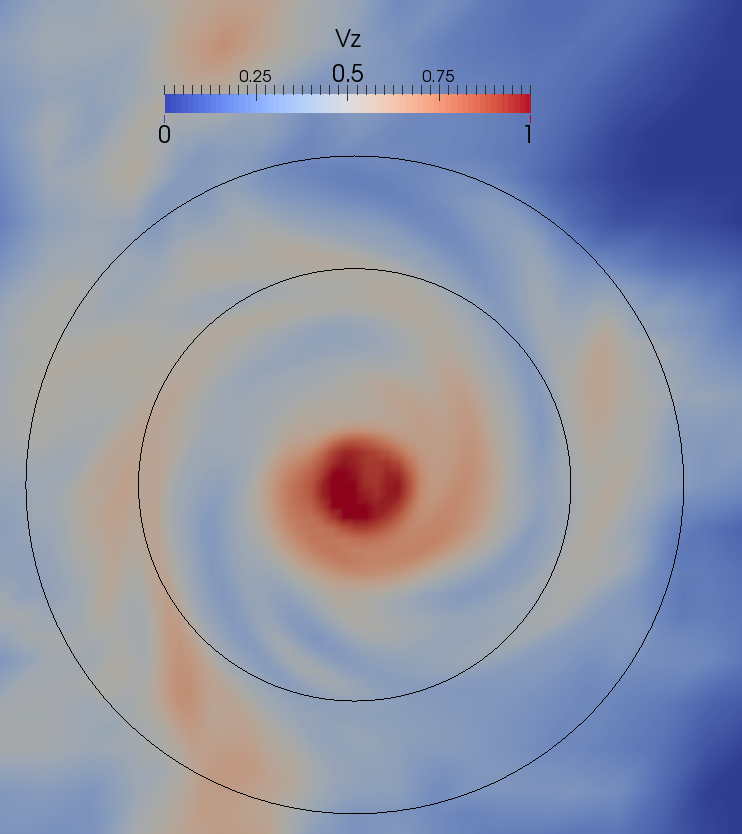
\includegraphics[width=.8\linewidth]{figs/vz_hor}
  \caption{Vertical Velocity}
  \label{fig:vz-to}
 \end{subfigure}%


 \begin{subfigure}{.5\textwidth}
  \centering
  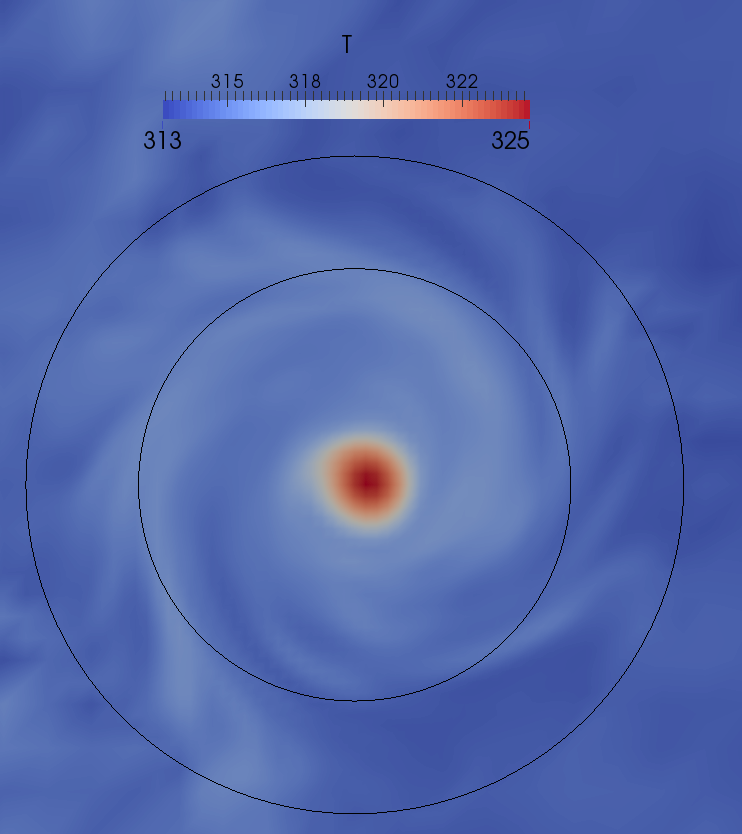
\includegraphics[width=.85\linewidth]{figs/t_hor}
  \caption{Temperature}
  \label{fig:t-to}
 \end{subfigure}%
 \begin{subfigure}{.5\textwidth}
  \centering
  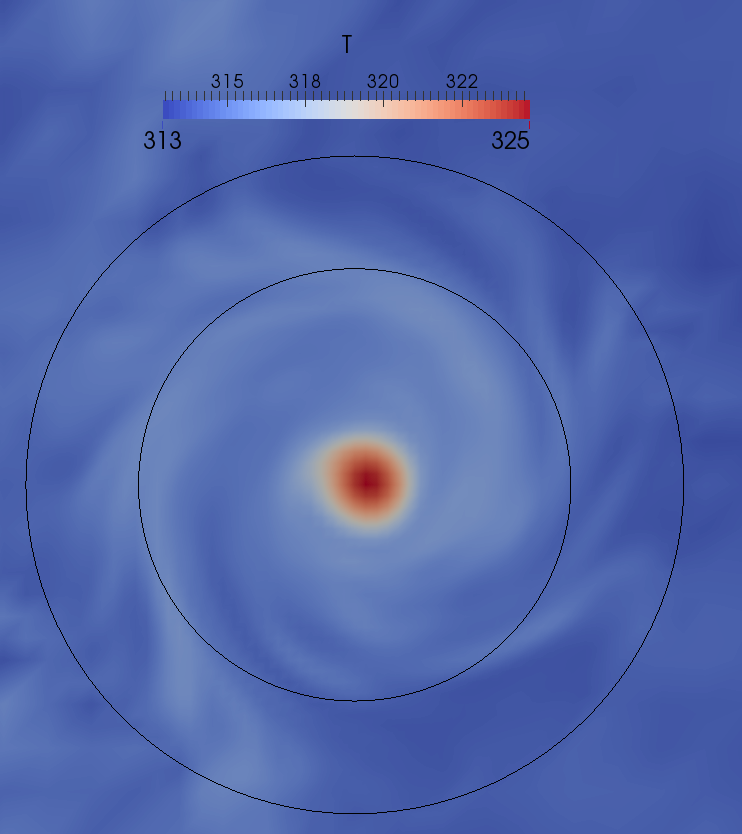
\includegraphics[width=.75\linewidth]{figs/t_hor}
  \caption{Pressure}
  \label{fig:p-to}
 \end{subfigure}%

 \caption{Horizontal slices for the thermal-only cases.}
 \label{fig:to-hor}
\end{figure}

Figure \ref{fig:to-hor}, depicts several horizontal slices
through the SoV for the same state variables. It can be seen that the
large velocities are highly localized to a region just inside the
vanes. Likewise, the entrainment of fluid is limited to a region
immediately surrounding the vanes. 
%
% conclusion of thermal only
%
Finally, the thermal plume is relatively
narrow compared to the diameter of the device. It is desirable to
broaden the thermal plume, as this would create a larger vertical
momentum flux and consequentally a larger kinetic energy flux. 
%% This will presumably
%% entrain more surrounding fluid, driving it through the vanes and
%% imparting kinetic energy to the flow. The kinetic energy grows as the
%% square of the radius, so any broadening of the vortex core can greatly
%% enhance the kinetic energy flux. 
The diameter of the thermal core is
therefore a critical flow characteristic in the thermal-only
conditions. However, a means of determing the thermal plume's thickness 
is not presently known. Regardless, these slices lend credibilty to the
notion that our turning vane configuration is generating something with
visible parallels to a naturally occurring dust devil.   

\subsection{Wind}

todo\todo{what case is this?}

%
% horizontal slices
%
\begin{figure}[htb]

 \begin{subfigure}{.5\textwidth}
  \centering
  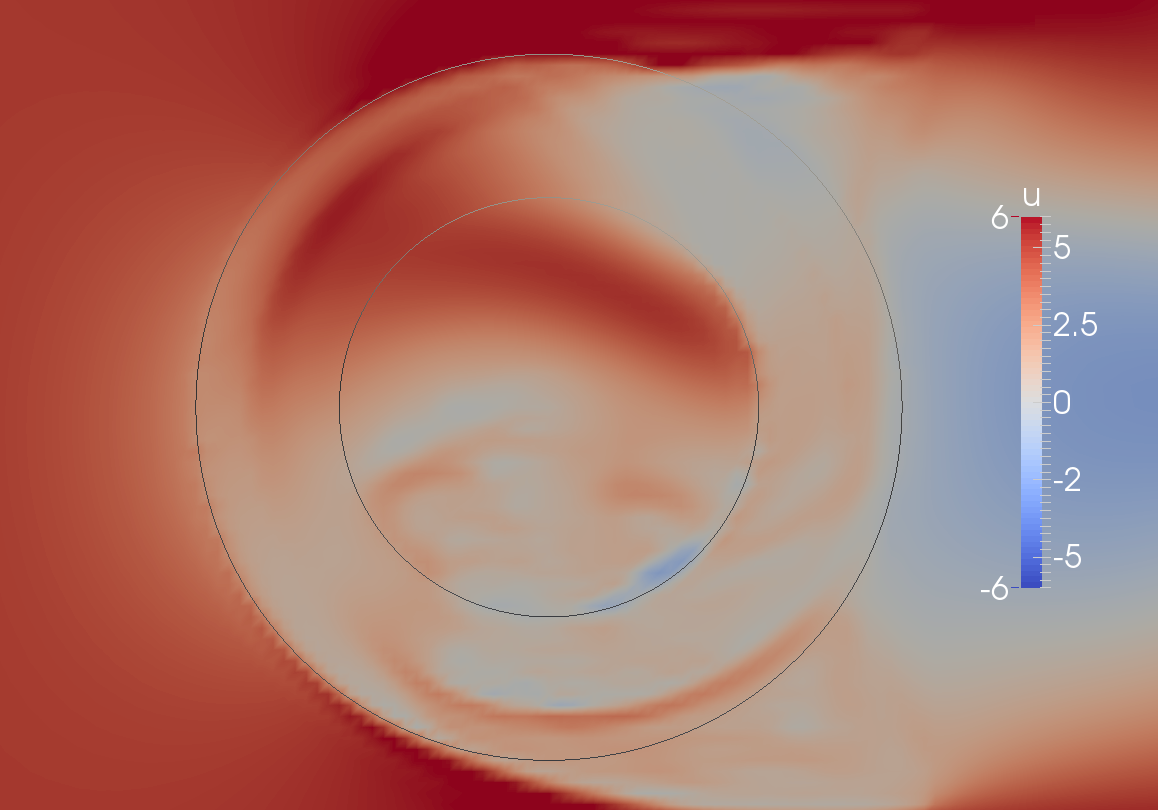
\includegraphics[width=.75\linewidth]{figs/wind_u}
  \caption{Streamwise}
  \label{fig:vt-wind}
 \end{subfigure}%
 \begin{subfigure}{.5\textwidth}
  \centering
  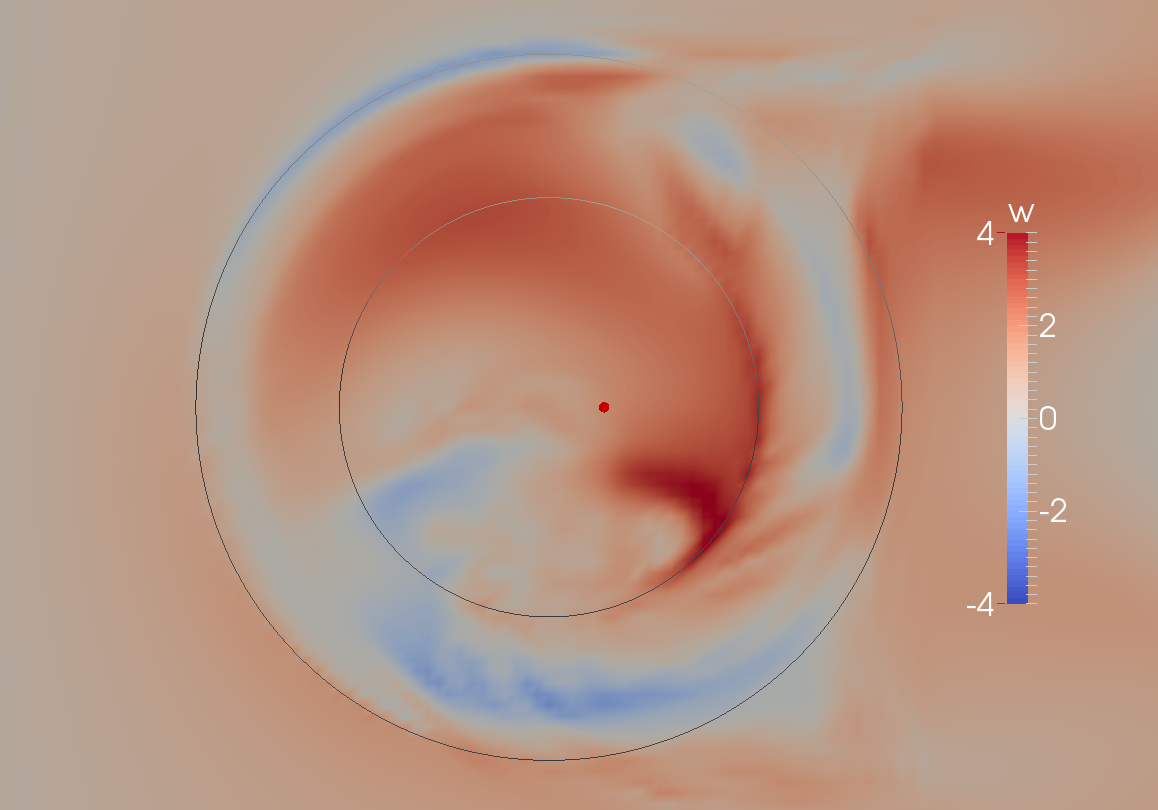
\includegraphics[width=.8\linewidth]{figs/wind_w}
  \caption{Vertical Velocity}
  \label{fig:vz-wind}
 \end{subfigure}%


 \begin{subfigure}{.5\textwidth}
  \centering
  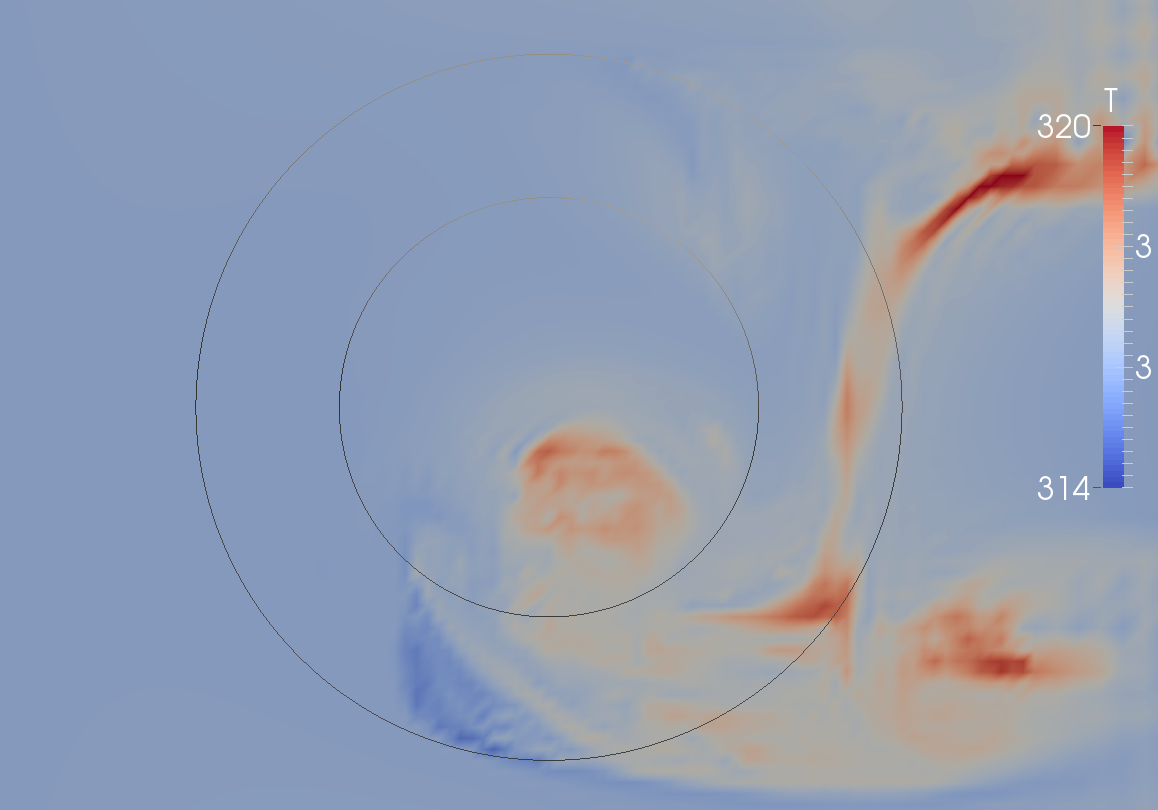
\includegraphics[width=.85\linewidth]{figs/wind_t}
  \caption{Temperature}
  \label{fig:t-wind}
 \end{subfigure}%
 \begin{subfigure}{.5\textwidth}
  \centering
  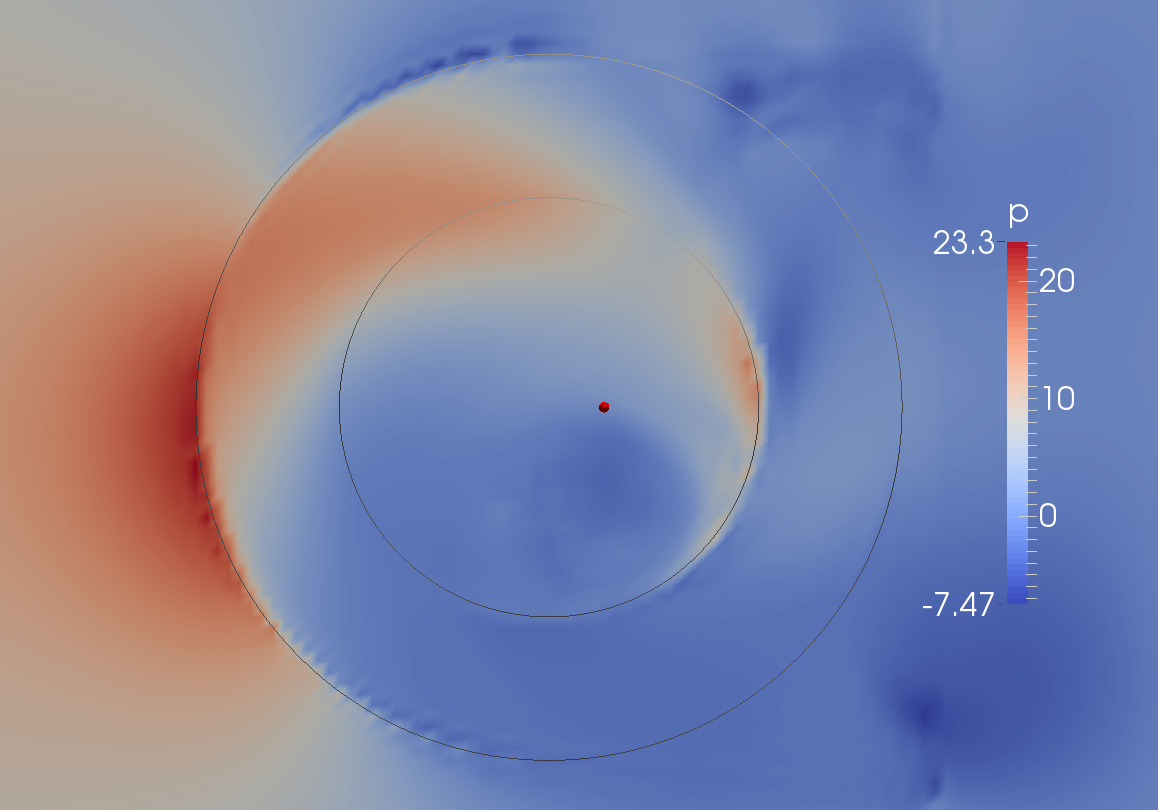
\includegraphics[width=.75\linewidth]{figs/wind_p}
  \caption{Pressure}
  \label{fig:p-wind}
 \end{subfigure}%

 \caption{Horizontal slices for the wind cases.}
 \label{fig:wind-hor}
\end{figure}


Horizontal slices of the azimuthal and vertical velocities, as well as the 
temperature and pressure fields are shown in figure
\ref{fig:vz-wind-vert}. The freestream velocity is traveling from left
to right at 5$ m/s$, which was set based on ambient velocity
measurements made by  the experimental team from the field. While the
structure is undoubtedly different than the thermal-only cases shown
previously, we can nevertheless see that a thermal plume is forming
along with a rotating velocity structure. In general the wind cases are
more disorganized, with less obviously visible coherent
structure. Notice however that the magnitude of velocities are several
times larger than  in the thermal-only cases, and the kinetic energy
flux through the vanes is also significantly higher.  

%
% vertical
%

\begin{figure}[htb]

 \begin{subfigure}{.5\textwidth}
  \centering
  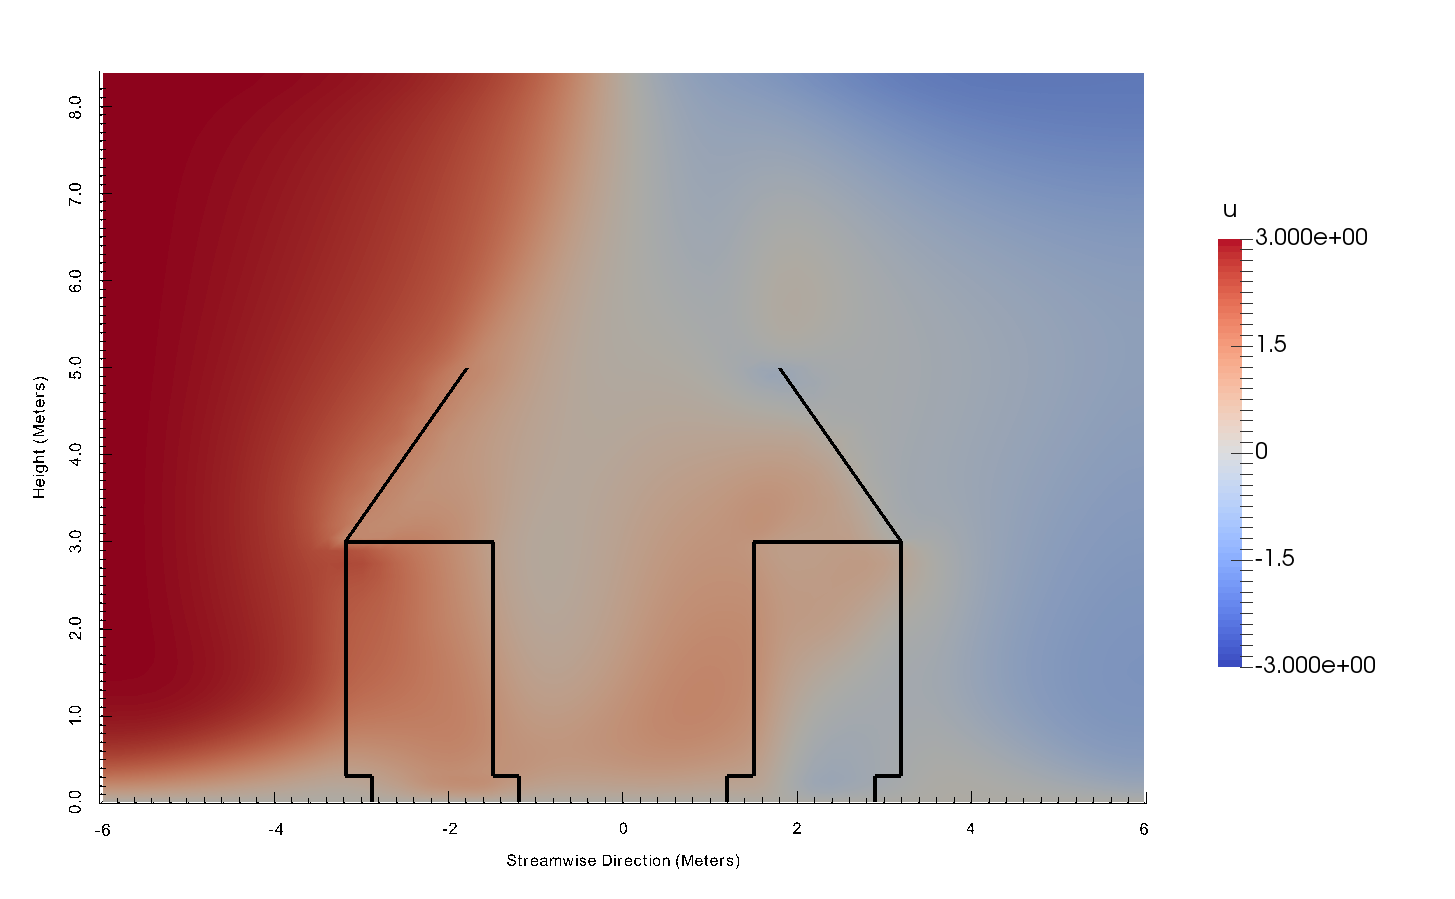
\includegraphics[width=.75\linewidth]{figs/wind_u_vertical}
  \caption{Streamwise}
  \label{fig:vt-wind-vert}
 \end{subfigure}%
 \begin{subfigure}{.5\textwidth}
  \centering
  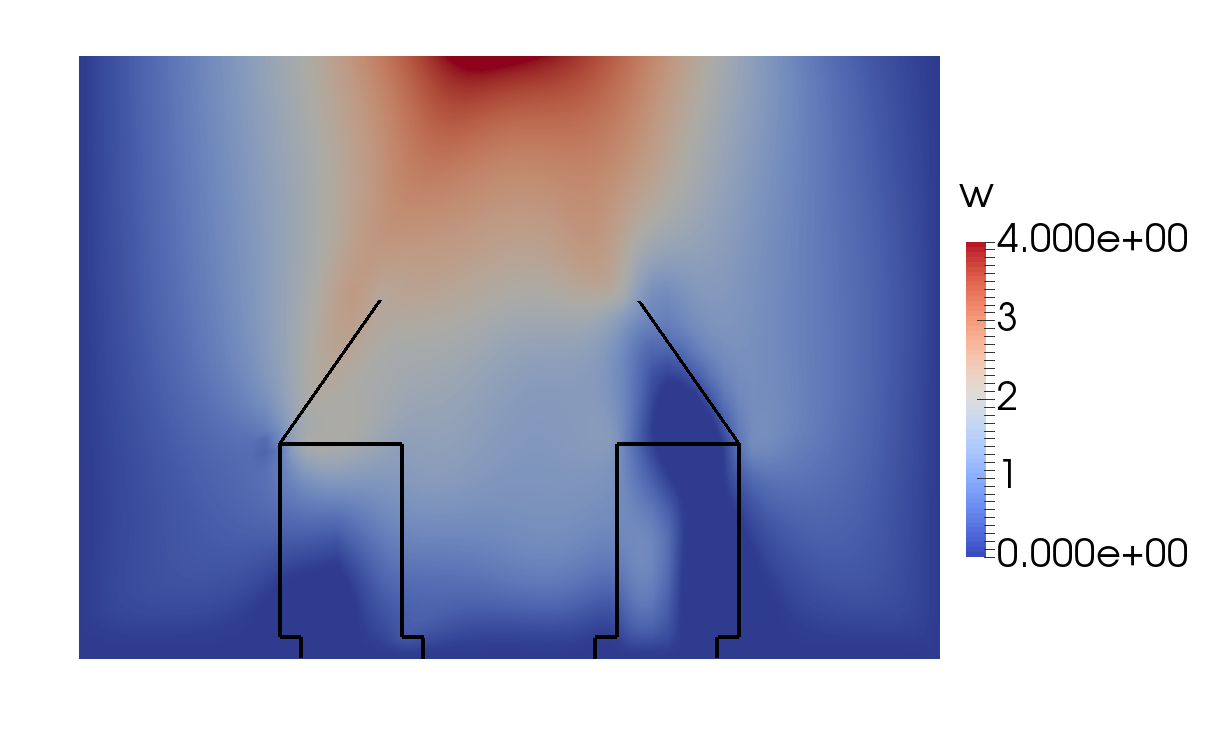
\includegraphics[width=.8\linewidth]{figs/wind_w_vertical}
  \caption{Vertical Velocity}
  \label{fig:vz-wind-vert}
 \end{subfigure}%


 \begin{subfigure}{.5\textwidth}
  \centering
  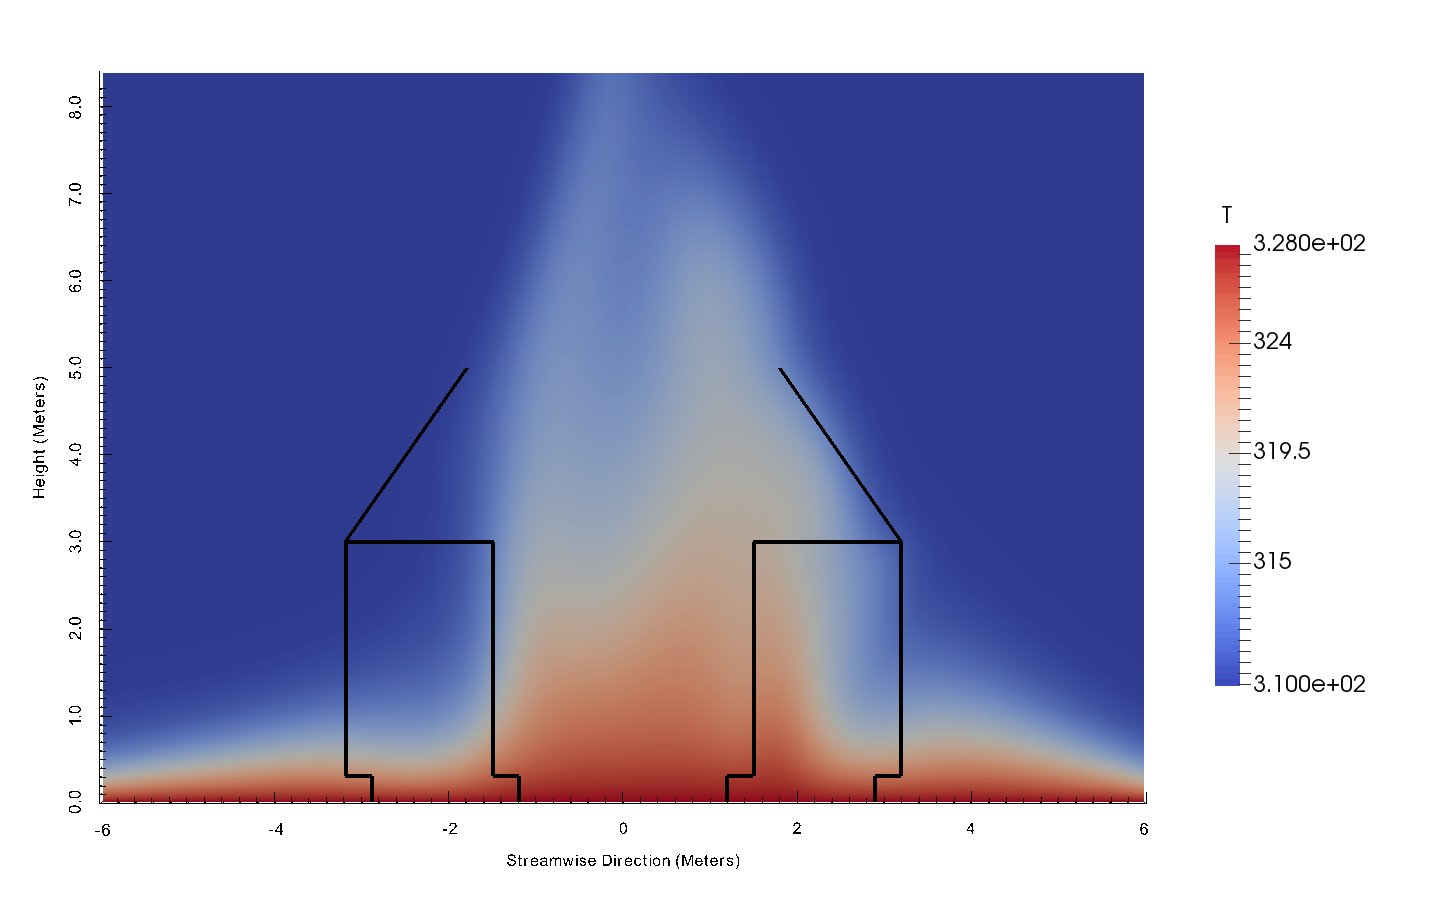
\includegraphics[width=.85\linewidth]{figs/wind_t_vertical}
  \caption{Temperature}
  \label{fig:t-wind-vert}
 \end{subfigure}%
 \begin{subfigure}{.5\textwidth}
  \centering
  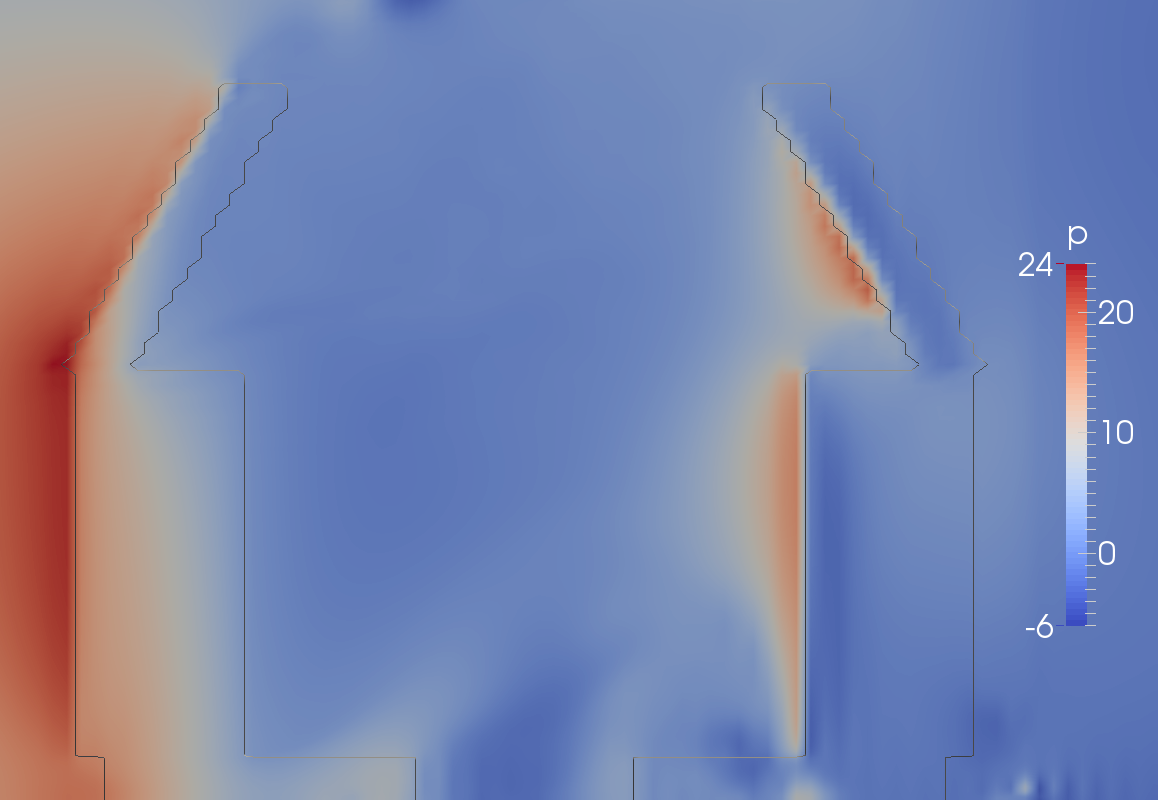
\includegraphics[width=.75\linewidth]{figs/wind_p_vertical}
  \caption{Pressure}
  \label{fig:p-wind-vert}
 \end{subfigure}%

 \caption{Vertical slices for the wind cases.}
 \label{fig:wind-ver}
\end{figure}

The vertical slices are shown in figure \ref{fig:wind-ver}. In this
case, the lower tier of vanes are where the majority of flow is 
entering the center of the apparatus, while the second tier of vanes are
blocking the ambient wind and providing protection to the vortex column. 

The thermal plume is significantly less
visible than in the thermal-only cases. While the
thermal-plume is necessarily weaker relative to the wind, some of this
is also due to the plume no longer being directly centered in the
flow. The plume is more visible using isocountors to render a
three-dimensional surface. 
To visualize the difference between the vertically varying ambient temperature
and the warmer thermal plume, we use the potential temperature, defined
as, 
\begin{equation}
  \tau(x,y,z) = T(x,y,z) -T_{in}(z) 
   \label{eqn:tau}
\end{equation}
where $T_{in}$ is the inflow temperature, described
in section \ref{sec:bc}. In this way the background potential
temperature is nearly zero, and larger values represent deviations from
the base flow temperature. The isocountour of a three Kelvin is 
shown in figure \ref{fig:field_real}. This value was selected as
it was noted as sufficient for formation of a dust devil by
Sinclair\cite{Sinclair1969}. It is clear from the image that a 
strong thermal column does exist even in the $5 m/s$ wind cases. 

%
% tiso
%
  \begin{figure}[!htb]
   \begin{center}
    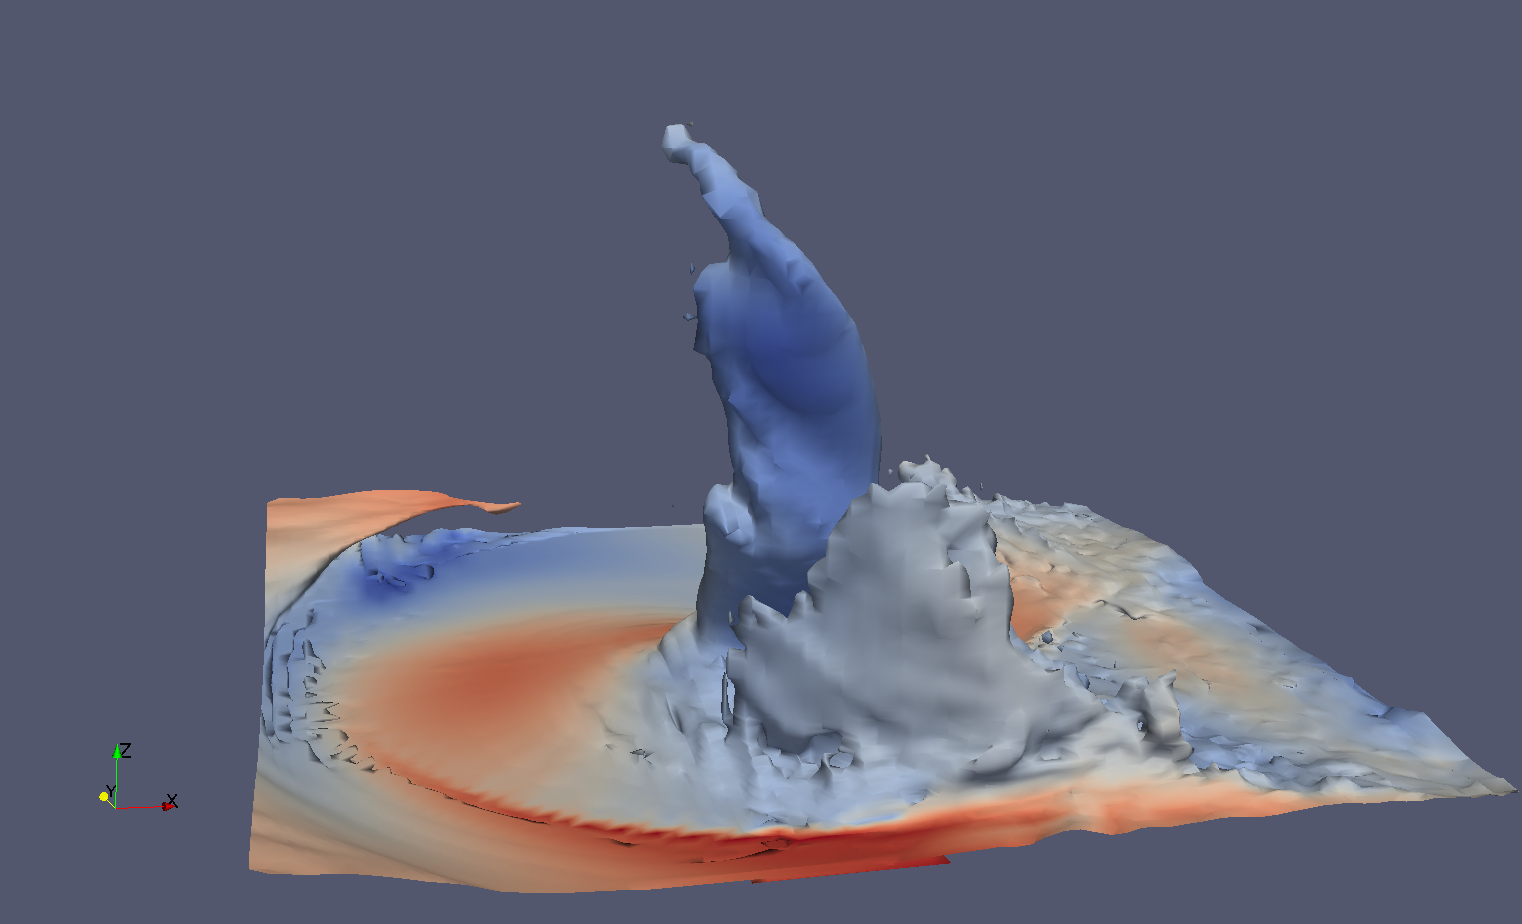
\includegraphics[width = 12 cm]{figs/t_iso}
    \caption{Isocountor of the thermal plume. Here, the isocontour is
    labelled by the potential temperature, $\tau$, as defined in \ref{eqn:tau}.(make this understandible!)}
    \label{fig:field_real}
   \end{center}
  \end{figure}

\subsection{Optimization}

In this section results from a representative optimization
in a thermal-only case are discussed, to demonstrate the optimization 
process employed so far. This is a typical mode of scientific and
engineering inquiry, where a hypothesis regarding system operation is
developed, followed by testing of the hypothesis, and further
iterations.  

This series of simulations are all runs with different system
configurations conducted in a common ambient scenario, that of the
unsteady thermal-only simulations described \todo{add pertinent bcs
here}. 

Our objective is to maximize the energy that can be 
extracted from the synthetic dust devil. As a surrogate to this
quantity, consider the kinetic energy flux through a horizontal plane
near the top of the vanes, where a turbine will ultimately be
placed. This is a surface integral\cite{landau1959fm}

%% \begin{equation}
%%  \dot E = -\oint \rho \textbf{v}(\frac{1}{2}v^2 + e) \cdot d \textbf{f}
%% \end{equation}
%% where $e$ is the internal energy. % and $d\textbf{f}$ the. 
%% For our problem, we consider an incompressible fluid flowing through a
%% flat horizontal region interior to the vanes in the x-y plane, which
%% results in, 

 \begin{equation}
 \dot E = -\frac{\rho }{2} \int V_z (V_{\theta}^2 + V_z^2 ) dA.
 \end{equation}

\begin{figure}[htb]
 \centering
 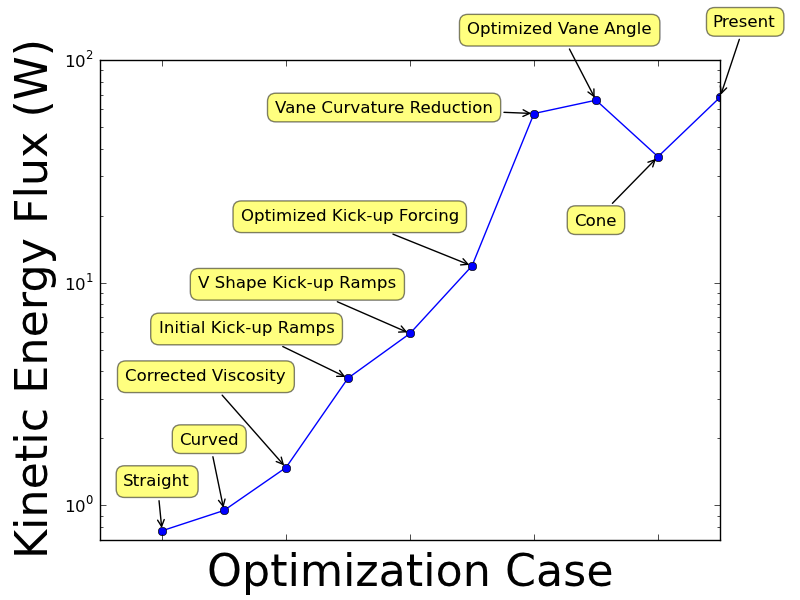
\includegraphics[width=.75\linewidth]{figs/opt_plot}
 \caption{This plot diagrams the improvements to the calculated flux for  
 each iteration of system configuration. Every iteration is labeled by
 design change.}
 \label{fig:opt_plot}
\end{figure}


\begin{figure}[htb!]
 \begin{subfigure}{.5\textwidth}
  \centering
  
\includegraphics[width=.75\linewidth]{figs/before_vanes}
  \caption{Vanes before optimization}
 \end{subfigure}%
 \begin{subfigure}{.5\textwidth}
  \centering
  
\includegraphics[width=.8\linewidth]{figs/after_vanes}
  \caption{Vanes after optimization}
 \end{subfigure}%
  \caption{Can we do this}
 \label{fig:vt-wind-vert}
\end{figure}\todo{need better figure}


%
%
\begin{figure}[htb!]
 \begin{subfigure}{.5\textwidth}
  \centering
  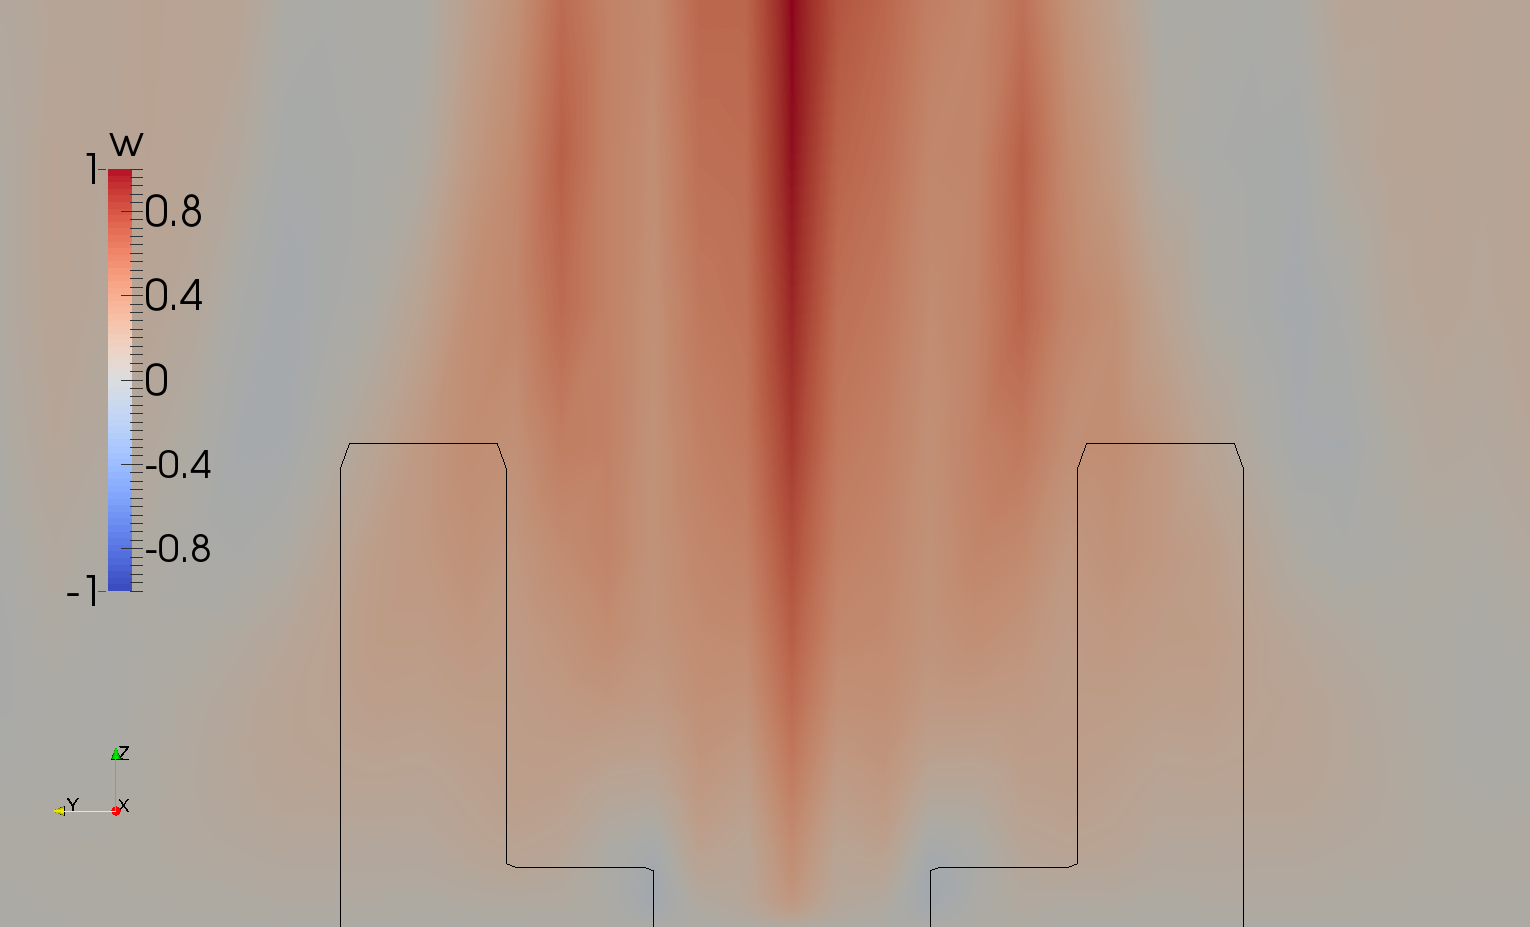
\includegraphics[width=.75\linewidth]{figs/before_opt}
  \caption{Flow before optimization}
 \end{subfigure}%
 \begin{subfigure}{.5\textwidth}
  \centering
  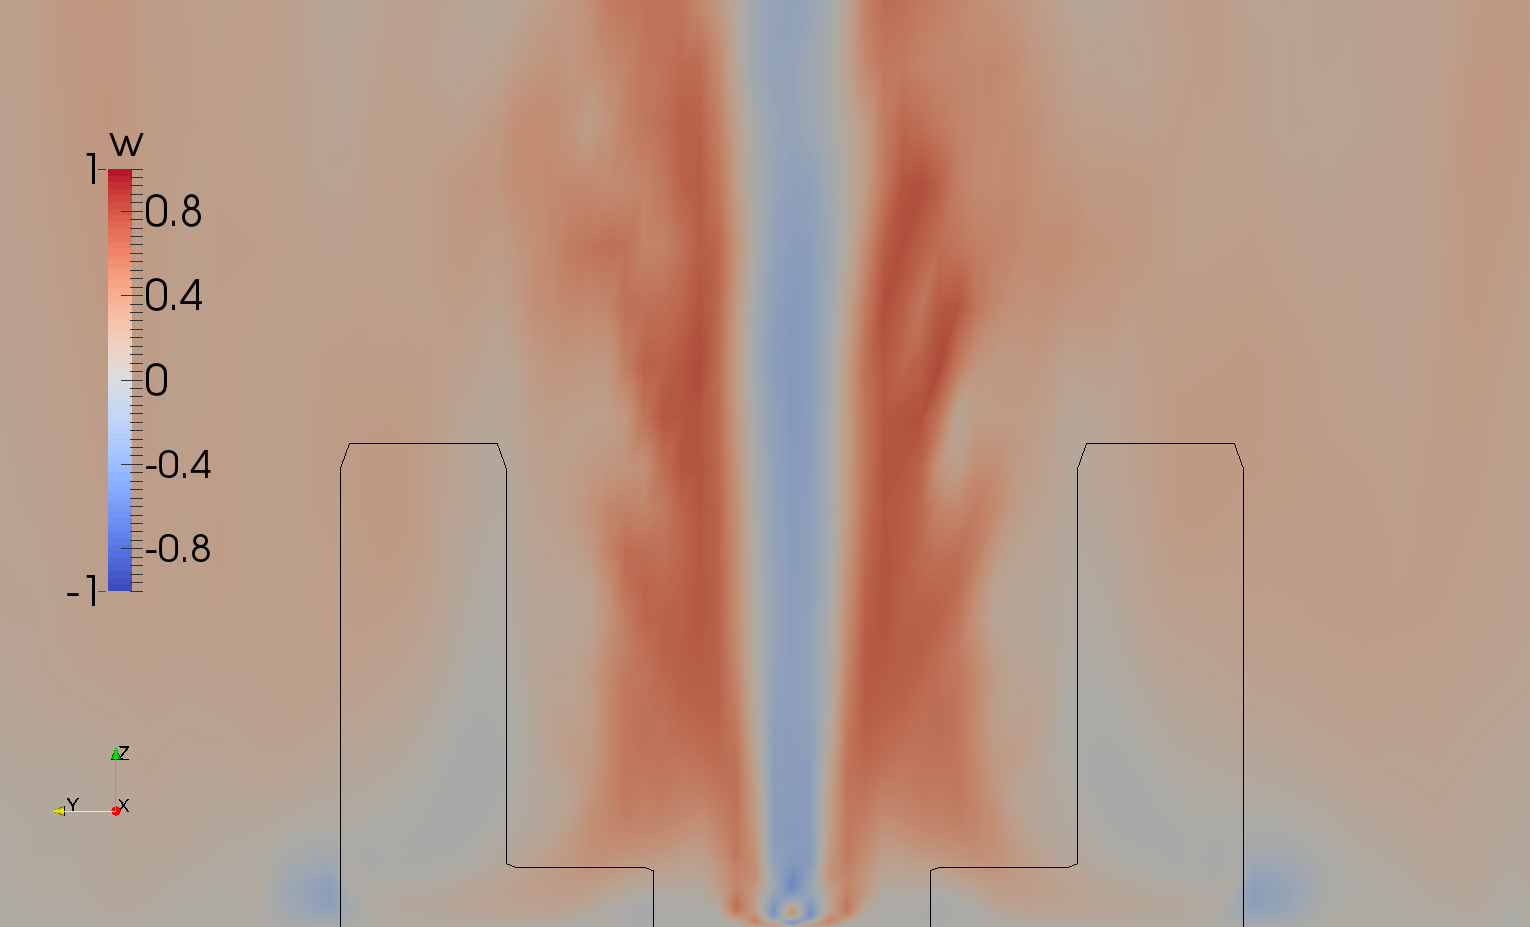
\includegraphics[width=.8\linewidth]{figs/after_opt}
  \caption{Flow after optimization}
 \end{subfigure}%
  \caption{Can we do this}
  \label{fig:opt_flow}
\end{figure}
%

Using the kinetic energy flux as an objective, the vane geometry has
been optimized. Over approximately tens of iterations, we have
increased the kinetic energy flux by a factor of 88 relative to the
baseline. Results of several of these iterations are documented in
figure \ref{fig:opt_plot}. Major adjustments to design in the the vane
shape and angles were made to obtain this improvement. Before and after
images shown in \ref{fig:vt-wind-vert}. During this optimization the
qualitative character of the solution changed substantially, changing
from a mild upward flow with little rotation to a strongly organized
vortex with a downward central flow and strong azimuthal
velocities. Before and after vertical slices are shown in figure
\ref{fig:opt_flow}. Nevertheless, with a peak energy flux for the final 
iteration of less than one hundred Watts, significant further
optimization is necessary for this system to be viable for use as an 
energy production system. This naturally precedes the next section,
which contains a discussion of the proposed research campaign and the
expected course of work that will be performed 

